\documentclass[20pt]{beamer}
% Colours come from colour brewer
\usepackage{xcolor}
\definecolor{b-blue}{HTML}{6baed6}
\definecolor{b-darkgrey}{HTML}{2D2D2D}
\definecolor{b-grey}{HTML}{969696}
\definecolor{b-purple}{HTML}{9e9ac8}
\definecolor{b-green}{HTML}{74c476}
\definecolor{b-pink}{HTML}{e377c2}
\definecolor{b-orange}{HTML}{FD8D3C}

\usepackage{relsize}

\usepackage{fontspec}
\defaultfontfeatures{Mapping=tex-text} % enable -- / --- / `` / ''
\setsansfont[ItalicFont={* Light},BoldItalicFont={* ExtraLight}]{Yanone Kaffeesatz}
\setmonofont[Scale=0.75]{Bitstream Vera Sans Mono}

% Neutralise underscores, since we don't use them apart for in URLs
\catcode`_=12
\begingroup\lccode`~=`_\lowercase{\endgroup\let~\sb}
\mathcode`_="8000

\usepackage{tikz}
\usetikzlibrary{positioning}
\usetikzlibrary{shapes.geometric}
\usetikzlibrary{calc}
% Useful for pictures.
\tikzstyle{nopadding} = [inner sep=0cm]
\tikzstyle{attribution} = [fill=b-darkgrey, anchor=south,
outer sep=0, inner sep=.1ex, font=\relsize{-6}\it,
minimum width=\paperwidth, text width=.95\paperwidth]
\tikzstyle{packages} = [fill=b-darkgrey, anchor=south,
outer sep=0, inner sep=.5ex, font=\relsize{-1},
minimum width=\paperwidth, text width=.95\paperwidth]

\newcommand{\hero}[1]{%
  \begin{tikzpicture}[remember picture, overlay]%
  \node[anchor=west,align=left,font=\Huge\bfseries] (A) at ($(current page.west) + (0.05\paperwidth, .17\paperheight)$) {%
    #1
  };
\end{tikzpicture}}

\newcommand{\herohigh}[1]{%
  \begin{tikzpicture}[remember picture, overlay]%
  \node[anchor=west,align=left,font=\Huge\bfseries] (A) at ($(current page.west) + (0.05\paperwidth, .25\paperheight)$) {%
    #1
  };
\end{tikzpicture}}

\newcommand{\heroveryhigh}[1]{%
  \begin{tikzpicture}[remember picture, overlay]%
  \node[anchor=north west,align=left,font=\Huge\bfseries] (A) at
  ($(current page.north west) + (0.05\paperwidth, -0.05\paperheight)$) {%
    #1
  };
\end{tikzpicture}}

\newcommand{\minionhigh}[1]{%
  \begin{tikzpicture}[remember picture, overlay]%
  \node[anchor=west,align=left,font=\Large\bfseries] (A) at ($(current page.west) + (0.05\paperwidth, .25\paperheight)$) {%
    #1
  };
\end{tikzpicture}}

\newcommand{\minionveryhigh}[1]{%
  \begin{tikzpicture}[remember picture, overlay]%
  \node[anchor=north west,align=left,font=\Large\bfseries] (A) at ($(current page.north west) + (0.05\paperwidth, -0.05\paperheight)$) {%
    #1
  };
\end{tikzpicture}}

\newcommand{\upperhalf}[1]{%
  \begin{tikzpicture}[remember picture, overlay]%
    \node[anchor=west,font=\normalsize, align=left] at
    ($(current page.west) + (0.05\paperwidth, .25\paperheight)$) {%
      #1
    };
  \end{tikzpicture}
}

\newcommand{\lowerhalf}[1]{%
  \begin{tikzpicture}[remember picture, overlay]%
    \node[anchor=west,font=\normalsize, align=left] at
    ($(current page.west) + (0.05\paperwidth, -.25\paperheight)$) {%
      #1
    };
  \end{tikzpicture}
}

\newcommand{\bottomhalf}[1]{%
  \begin{tikzpicture}[remember picture, overlay]%
    \node[anchor=south west,font=\normalsize, align=left] at
    ($(current page.south west) + (0.05\paperwidth, 0)$) {%
      #1
    };
  \end{tikzpicture}
}

\newcommand{\inthemiddle}[1]{%
  \begin{tikzpicture}[remember picture, overlay]%
    \node at (current page.center) {%
      #1
    };
  \end{tikzpicture}
}

\newcommand{\bottomleft}[1]{%
  \begin{tikzpicture}[remember picture, overlay]%
    \node[anchor=south west, align=left,font=\footnotesize] at (current page.south west) {%
      #1
    };
  \end{tikzpicture}
}

\newcommand{\bottomright}[1]{%
  \begin{tikzpicture}[remember picture, overlay]%
    \node[anchor=south east, align=right,font=\footnotesize] at (current page.south east) {%
      #1
    };
  \end{tikzpicture}
}

\newcommand{\bottomhanging}[1]{%
  \begin{tikzpicture}[remember picture, overlay]%
    \node[anchor=north] at
    ($(current page.center) + (0, .17\paperheight)$) {
      #1
    };
  \end{tikzpicture}
}

\newcommand{\bottomhangingverylow}[1]{%
  \begin{tikzpicture}[remember picture, overlay]%
    \node[anchor=north] at
    ($(current page.center) + (0, -0.05\paperheight)$) {
      #1
    };
  \end{tikzpicture}
}

\newcommand{\bottomhanginghigh}[1]{%
  \begin{tikzpicture}[remember picture, overlay]%
    \node[anchor=north] at
    ($(current page.center) + (0, .24\paperheight)$) {
      #1
    };
  \end{tikzpicture}
}

\newcommand{\bottomhanginglow}[1]{%
  \begin{tikzpicture}[remember picture, overlay]%
    \node[anchor=north] at
    ($(current page.center) + (0, .1\paperheight)$) {
      #1
    };
  \end{tikzpicture}
}

\newcommand{\bottomhangingleft}[1]{%
  \begin{tikzpicture}[remember picture, overlay]%
    \node[anchor=north west,align=left] at
    ($(current page.west) + (0.05\paperwidth, .17\paperheight)$) {
      #1
    };
  \end{tikzpicture}
}


% Missing so far:
%
% 1. Something about my context (who am I to talk about this?)
% 2. Something more broadly about the problems - real use cases?
%    - perhaps something on the R data package
%    - perhaps something about dat project too
%    - taxonlooup as an example of this

\usepackage{fontawesome}
\newfontfamily{\FA}{FontAwesome}
\def\twitter{{\FA \faTwitter}}
\def\github{{\FA \faGithub}}
\def\heart{{\FA \faHeart}}
\def\tickmark{{\FA \faCheck}}
\def\rarrow{{\FA \relsize{-1}{\faArrowRight}}}
\def\imagetop#1{\vtop{\null\hbox{#1}}}
\def\code{\texttt}
\newcommand{\hrefp}[2]{\href{#1://#2}{#2}}
\newcommand{\twitterhandle}[1]{\href{https://twitter.com/#1}{#1}}
\newcommand{\ghrepo}[1]{\href{https://github.com/#1}{\tt github.com/#1}}
\newcommand{\twitterhandlesm}[1]{\relsize{-1}{\color{b-grey}\href{https://twitter.com/#1}{@#1}}}

\begin{document}

\setbeamercolor*{palette primary}{fg=white,bg=b-darkgrey}
\setbeamercolor*{titlelike}{parent=palette primary}
\setbeamercolor*{normal text}{parent=palette primary}
\setbeamercolor*{itemize}{parent=palette primary}
\color{white}
\setbeamertemplate{navigation symbols}{}
\setbeamercolor{itemize/enumerate body}{fg=white}
\setbeamercolor{enumerate item}{fg=white}
\setbeamertemplate{itemize item}{\raisebox{.33ex}{\footnotesize\color{white}$\blacktriangleright$}}

\begin{frame}
  \begin{tikzpicture}[remember picture, overlay]
    \node (A) at ($(current page.center) + (0, .17\paperheight)$) {
      \resizebox{.9\paperwidth}{!}{%
        \color{b-blue}\bf Tools for collaborative data use}
    };
    \node[anchor=north] at (A.south) {
      \resizebox{.9\paperwidth}{!}{%
        \color{b-green}\ldots for users who do not want to care}
    };
    \color{white}
    \node[anchor=south west] (B) at
    ($(current page.south west) + (0.05\paperwidth, 0.05\paperwidth)$) {
      \color{b-grey}\twitter\ \twitterhandle{rgfitzjohn}%
      \hspace{.07\textwidth}%
      \color{b-grey}\github\ \href{https://github.com/richfitz}{richfitz}
    };
    \node[anchor=south west] at (B.north west) {
      Rich FitzJohn, Imperial College London
    };
  \end{tikzpicture}
\end{frame}

% Some background about me, Imperial, people's skills and how we get
% to this point.

% Also need to get across that the tools that I will present are super
% new.  They're not being widely used within the department yet
% because I'm still trying to scope what the problems are and how we
% can solve them.

\begin{frame}
  \herohigh{\color{b-blue}Two related problems}
  \bottomhanginglow {
    \begin{minipage}{\textwidth}
      \begin{itemize}
      \item Data distribution \& versioning
      \item Sharing sensitive data
      \end{itemize}
    \end{minipage}}
\end{frame}

% Get a picture of a "data deluge", and then go into some more detail
% about the sorts of data that people have.  1mb excel files and other
% relatively innocent things are an issue here.

% * We love git
% * But it sucks for data
%   - git annex (wtf is going on there)
%   - git lfs (needs a server)
%   - many others
%   - dat, at some point in the future, could be very exciting.
%
%   Version control of data is hard!  Dat will solve the problem but I
%   have been waiting for it do so for ages, and they're mostly
%   interested in massively multiuser tabular data, rather than things
%   that scientists use, such as trees, database dumps, shapefiles,
%   whatever.
%
%   Because git is so central to New Science it all gets a bit
%   derailed when you hit any data of real size.
{
  \setbeamercolor{background canvas}{bg=white}
  \begin{frame}
    \begin{tikzpicture}[remember picture, overlay]%
      \node (A) at (current page.center) {%
        \includegraphics[width=\textwidth]{snippets/bigdata}
      };
      \node[anchor=north east] (B) at
      ($(A.south east) + (0, .075\paperheight)$) {%
        \only<1>{\color{b-pink}lol jk}%
        \only<2>{\color{b-blue}\LARGE \ldots for git}%
      };
    \end{tikzpicture}
  \end{frame}
}

\begin{frame}
  \herohigh{\color{b-pink}Data versioning}
  \bottomhanginglow{%
    \raisebox{-.07\paperheight}{
\includegraphics[height=.15\paperheight]{pics/logos/git}}%
    \hspace{.025\paperwidth}{\LARGE +}\hspace{.03\paperwidth}%
    \raisebox{-.07\paperheight}{%
      \includegraphics<1>[height=.15\paperheight]{pics/code}%
      \includegraphics<2>[height=.15\paperheight]{pics/database_icon1}%
      \includegraphics<3>[height=.15\paperheight]{pics/database_icon3}%
      \includegraphics<4>[height=.15\paperheight]{pics/database_icon5}}%
    \hspace{.025\paperwidth}{\LARGE =}\hspace{.03\paperwidth}%
    \raisebox{-.1\paperheight}{%
      \includegraphics<1>[height=.20\paperheight]{pics/rage0}%
      \includegraphics<2>[height=.20\paperheight]{pics/rage1}%
      \includegraphics<3>[height=.20\paperheight]{pics/rage3}%
      \includegraphics<4>[height=.20\paperheight]{pics/rage5}}%
  }
\end{frame}

% The usual solution proposed here is "just put it on figshare" or
% some other service.  But this solves only one of the set of
% problems.
\begin{frame}
  \hero{\color{b-green}``Just put it on}
  \begin{tikzpicture}[remember picture, overlay]%
    \node[anchor=east,align=right,font=\Huge\bfseries] (A) at ($(current page.east) + (-0.15\paperwidth, -.05\paperheight)$) {%
      \only<1>{dropbox''}%
      \only<2>{figshare''}%
    };
  \end{tikzpicture}
\end{frame}

\begin{frame}
  \minionhigh{\color{b-pink}How do we\ldots}
  \bottomhanging {
    \begin{minipage}{\textwidth}
      \begin{itemize}
      \item store the potentially large(ish) data?
        \only<2>{{\color{b-green}\tickmark}}\vphantom{\tickmark}
      \item load the data into R?
      \item work offline / cache reads?
      \item deal with multiple versions?
      \item control access to the data?
      \end{itemize}
    \end{minipage}}
\end{frame}

\begin{frame}
  \hero{\color{b-blue} datastorr}
  \bottomhangingverylow{\ghrepo{richfitz/datastorr}}
\end{frame}

% Here, I should show how this works in practice.  The key ingredients
% are:
%
% Store data against gh releases.
\begin{frame}
  \minionhigh{\color{b-blue}Storage: \color{b-green}GitHub releases}
  % Include a screenshot here I think.  Probably of baad or datastorr
  \bottomhanginglow{
    \begin{minipage}{.94\textwidth}
      \color{white}\raggedright
      ``We don't limit the total size of your binary release files, nor
      the bandwidth used to deliver them. However, each individual
      file must be under {\color{b-pink}2GB} in size.''
    \end{minipage}}
  \bottomright{\tt help.github.com/articles/distributing-large-binaries}
\end{frame}

\begin{frame}
  \minionhigh{\color{b-blue}Storage: \color{b-green}GitHub releases}
  \bottomhanging{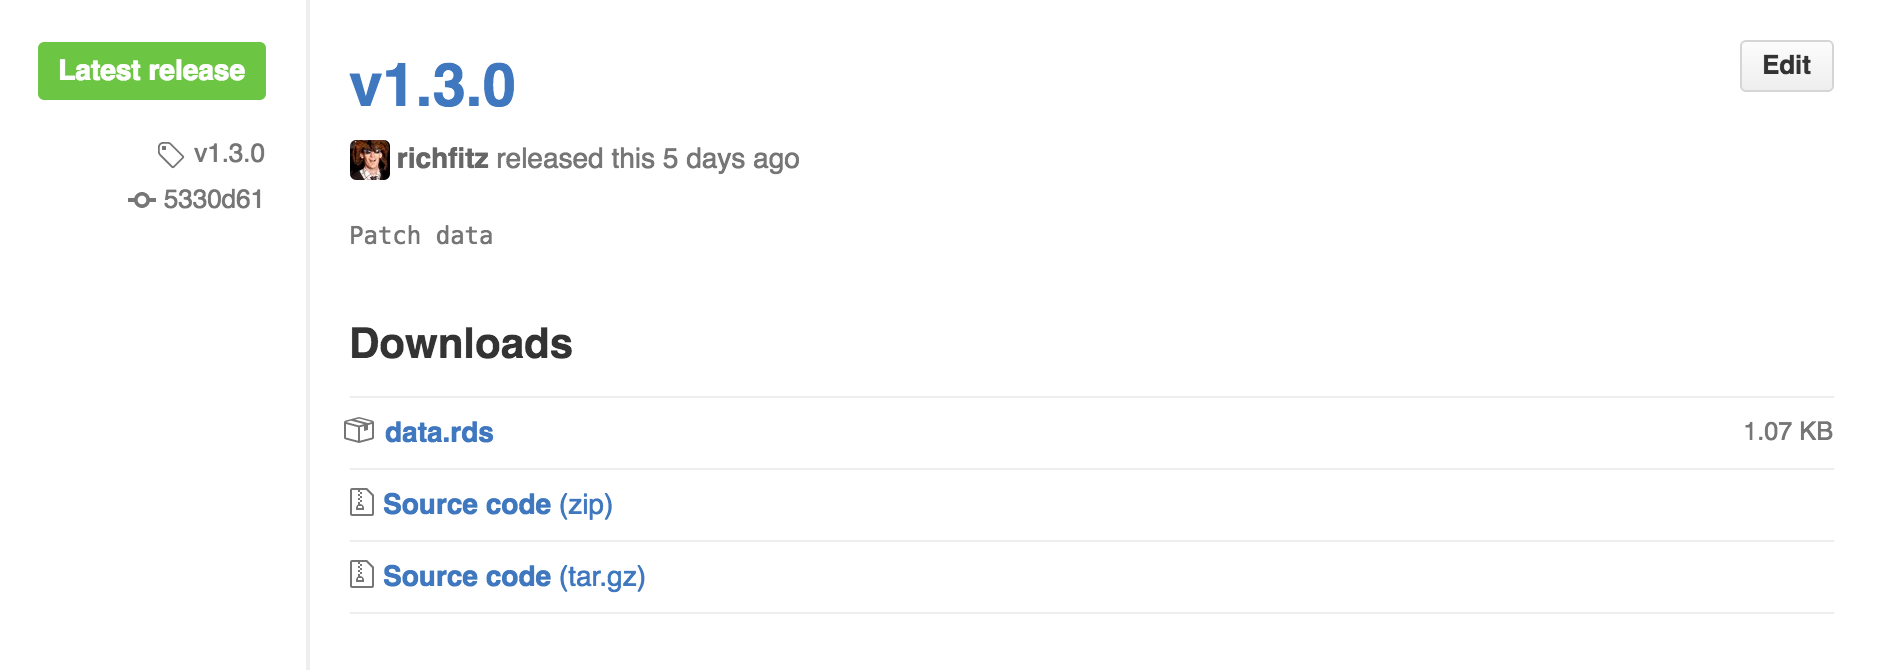
\includegraphics[width=\textwidth]{pics/shots/releases-gh}}
  \bottomright{\ghrepo{richfitz/data/releases}}
\end{frame}

\begin{frame}
  \minionhigh{\color{b-blue} Configuration: \tt\color{b-green} datastorr.json}
  \bottomhanging{%
    \includegraphics<1>[width=.8\textwidth]{snippets/datastorr-json}}
  \bottomright{\ghrepo{richfitz/data}}
\end{frame}

% At this point we'll skip over how things get into the releases and
% work with the data assuming that they're there.  I'll loop back to
% show how we put the data up there once the benefits of doing so are
% more obvious.

% At this point it might be worth showing how curl actually works here?
\begin{frame}
  \minionhigh{\color{b-blue}Transfer: \color{b-green}\texttt{curl} \& \texttt{httr}}
  \bottomhanging{
    \begin{minipage}{\textwidth}
      \includegraphics<1>[width=\textwidth]{snippets/datastorr-transfer-1}
      \includegraphics<2>[width=\textwidth]{snippets/datastorr-transfer-2}
      \includegraphics<3>[width=\textwidth]{snippets/datastorr-transfer-3}
    \end{minipage}}
  \bottomright{
    \begin{minipage}{\textwidth}
      \raggedleft
      \ghrepo{jeroenooms/curl}\\\ghrepo{hadley/httr}
    \end{minipage}
  }
\end{frame}

\begin{frame}
  \minionhigh{\color{b-blue}Caching: \color{b-green}\texttt{storr}}
  % Diagram with storr showing the caching layer(s)
  % Cloud -> Disk -> Environment -> R object
  \bottomhanging{
\includegraphics[width=\textwidth]{diagrams/datastorr}}
  \bottomright{\ghrepo{richfitz/storr}}
\end{frame}

\begin{frame}
  \minionhigh{\color{b-blue}Versioning:
    \color{b-green}\texttt{datastorr} \&
    \color{b-green}\texttt{storr}}
  \bottomhanging{
    \includegraphics<1>[width=\textwidth]{snippets/datastorr-version-1}
    \includegraphics<2>[width=\textwidth]{snippets/datastorr-version-2}
    \includegraphics<3>[width=\textwidth]{snippets/datastorr-version-3}
    \includegraphics<4>[width=\textwidth]{pics/shots/daff}
  }
  \bottomright{%
    \only<1-3>{\ghrepo{richfitz/datastorr}}%
    \only<4>{\ghrepo{edwindj/daff}}}
\end{frame}

\begin{frame}
  \minionhigh{\color{b-blue}Versioning: \color{b-green}semver.org}
  \bottomhanging{
    \begin{minipage}{1.0\linewidth}
      \begin{itemize}
      \item \texttt{{\color{b-pink}<major>}.{\color{b-blue}<minor>}.{\color{b-green}<patch>}}
      \item \textbf{\color{b-green} patch number}: new data, small updates
      \item \textbf{\color{b-blue} minor number}: new columns, big updates
      \item \textbf{\color{b-pink} major number}: breaking changes
      \end{itemize}
    \end{minipage}}
\end{frame}

{
  \setbeamercolor{background canvas}{bg=white}
  \begin{frame}
    \inthemiddle{%
      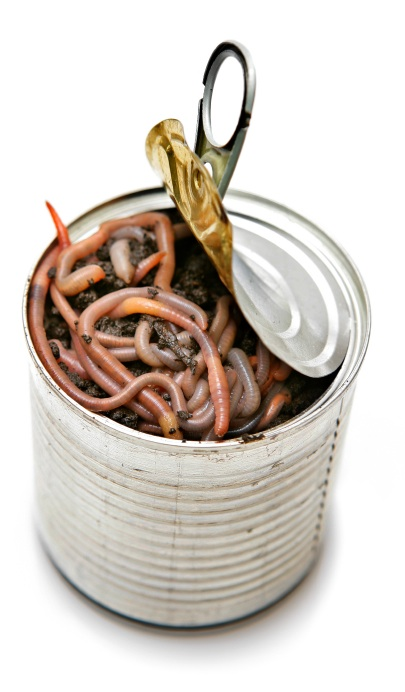
\includegraphics[height=.9\textheight]{pics/can-of-worms}}
  \end{frame}
}

\begin{frame}
  \minionhigh{\color{b-blue}Access control}
  \begin{minipage}{1.0\linewidth}
    \begin{itemize}
    \item Private repos = private data {\color{b-pink}{\FA \faLock}}
    \item Access with {\color{b-green}OAuth} or {\color{b-green}GitHub token} {\color{b-pink}{\FA
          \faUnlock}}
    \item Private organisation repos, too
    \end{itemize}
  \end{minipage}
\end{frame}


% I may need to wind it back a bit here; these are all the possible
% features of the package, and I do want to emphasise that this is
% meant to work well with the simple csv-as-moving-target use-case.
% So perhaps the creation part should be really simple.  I should
% point at an entire workflow here; a document or something that walks
% through the whole thing end-to-end.
\begin{frame}
  \herohigh{\color{b-orange}Making releases}
  \bottomhanginglow{
    \includegraphics<1>[width=\textwidth]{snippets/datastorr-release}}
\end{frame}

\begin{frame}
  \herohigh{\color{b-orange}Making releases}
  \bottomhanginglow{
    \begin{minipage}{1.0\linewidth}
      \begin{enumerate}
        \item Fetches metadata
        \item Checks remote version
        \item Creates remote tag
        \item Uploads file to releases
      \end{enumerate}
    \end{minipage}}
\end{frame}

\begin{frame}
  \minionhigh{\color{b-green}Next level: data packages}
  \begin{minipage}{1.0\linewidth}
    \begin{itemize}
    \item Dependency installation
    \item Post-processing
    \end{itemize}
  \end{minipage}
  \bottomright{\ghrepo{traitecoevo/taxonlookup}}
\end{frame}

% Perhaps offer an interactive bit

\begin{frame}
  \minionhigh{\color{b-pink}Data versioning}
  \bottomhanging {
    \begin{minipage}{\textwidth}
      \begin{itemize}
      \item store the potentially large data?
      \item load the data into R?
      \item work offline / cache reads?
      \item deal with multiple versions?
      \item control access to the data?
      \end{itemize}
    \end{minipage}}
  \bottomright{\tt github.com/richfitz/datastorr}
\end{frame}

\begin{frame}
  \begin{tikzpicture}[remember picture, overlay]
    \node[inner sep=0, outer sep=0] at (current page.center) {%
      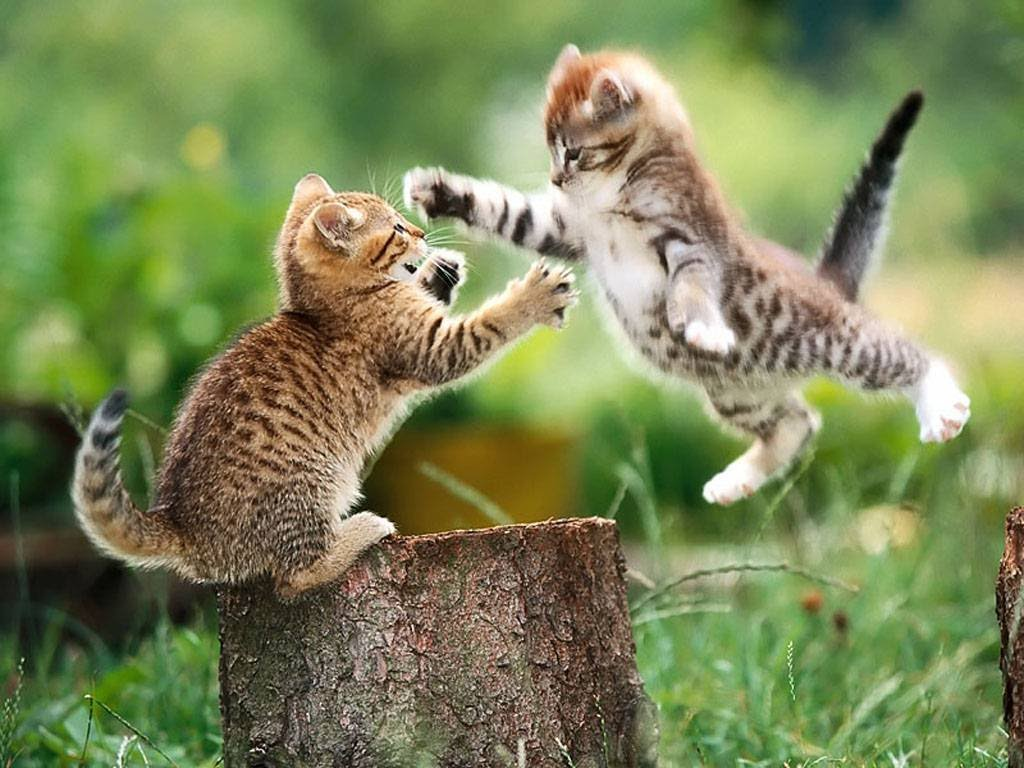
\includegraphics[width=\paperwidth]{pics/cat}};
  \end{tikzpicture}
\end{frame}

% Picture of a cute cat.

\begin{frame}
  \hero{\color{b-blue} Sensitive data}
\end{frame}

% There are two parts here I want to discuss.  The first is encryption
% aimed at *users* rather than at encryption dorks.  The second is the
% workflow for dealing with shared encrypted data in a sane way.

% I need something here that shows the scope of the problem -- there a
% bunch of different strands here:
%
% * storing senstive data in a public place (e.g., github)
% * storing data in a private place but risking leakage (e.g.,
%   computer loss/theft)
%
% because this is an area that is largely out of scope for biology so
% far I don't know what the full set of use-cases looks like.  It
% might be very limited, or very broad, but without the tooling it's
% going to be hard to tell.

% Be clear that we're not looking for some sort of internet banking
% solution where we have end-to-end security, where all secure
% calculations happen in encrypted memory -- we're after something
% simple where people's laptops might get stolen the data will not be
% lost.

\begin{frame}
  \minionhigh{Humane encryption}
  \bottomhanging{
    \includegraphics<1>[width=\textwidth]{snippets/cyphr-interface-1}%
    \includegraphics<2>[width=\textwidth]{snippets/cyphr-interface-2}%
    \includegraphics<3>[width=\textwidth]{snippets/cyphr-interface-3}%
    \includegraphics<4>[width=\textwidth]{snippets/cyphr-interface-4}%
    \includegraphics<5>[width=\textwidth]{snippets/cyphr-interface-other}%
  }
\end{frame}

\begin{frame}
  \minionhigh{\color{b-blue}Supported libraries}
  \bottomhanging {
    \begin{minipage}{\textwidth}
      \begin{itemize}
      \item OpenSSL - asymmetric
      \item Sodium - symmetric
      \item Sodium - asymmetric
      \item Sodium - authenticated
      \end{itemize}
    \end{minipage}
  }
  \bottomright{
    \begin{minipage}{\textwidth}
      \raggedleft
      \ghrepo{jeroenooms/openssl}\\\ghrepo{jeroenooms/sodium}
    \end{minipage}
  }
\end{frame}

\begin{frame}
  \minionhigh{\color{b-pink}How do we\ldots}
  \bottomhanging {
    \begin{minipage}{\textwidth}
      \begin{itemize}
      \item encrypt something?
        \only<2>{{\color{b-green}\tickmark}}\vphantom{\tickmark}
      \item share keys amongst users?
      \item \ldots so the key is not exposed?
      \item grant access to new people?
      \end{itemize}
    \end{minipage}}
\end{frame}

% Show a symmetric key (a circle) and that we can encrypt and decrypt
% with it.  Show this with little equations and with code/pseudocode.

\begin{frame}
  \minionveryhigh{\color{b-blue}Symmetric encryption}
  \bottomhanginghigh{\only<1>{%
      \begin{minipage}{\textwidth}
        \begin{itemize}
        \item Same key to encrypt and decrypt
        \item Everyone has the same key
        \end{itemize}
      \end{minipage}}
    \includegraphics<2>[width=.95\textwidth]{diagrams/encryption-sym-1}
    \includegraphics<3>[width=.95\textwidth]{diagrams/encryption-sym-2}}
\end{frame}

% The issue at this point is that it's not clear how we store the key.
% We obviously can't store it with the data because then it's
% basically all plain text.  We also have an issue distributing the
% key because it should be kept secret.  This is a building block for
% other methods.

\begin{frame}
  \minionveryhigh{\color{b-blue}Asymmetric (public key) encryption}
  \bottomhanging{\only<1>{%
    \begin{minipage}{\textwidth}
      \begin{itemize}
      \item Keys come in a pair (public and private)
      \item Anyone can encrypt a message with your public key
      \item You can decrypt it with your private key
      \end{itemize}
    \end{minipage}}
  \includegraphics<2>[width=.95\textwidth]{diagrams/encryption-asym}}
\end{frame}

% This is the first stage here
\begin{frame}
  \minionhigh{\color{b-blue}A workflow}
  \bottomhanging{\only<1>{%
      \begin{minipage}{\textwidth}
        \begin{enumerate}
        \item Generate SSH keys: \texttt{ssh-keygen}
        \item Generate a symmetric key for the data
        \item Encrypt data key with your SSH public key
        \item Store encrypted key somewhere
        \end{enumerate}
      \end{minipage}}
    \includegraphics<2>[width=.85\textwidth]{diagrams/encryption-asym}%
    \includegraphics<3>[width=.85\textwidth]{diagrams/encryption-workflow}}
  \bottomright{\ghrepo{richfitz/cyphr}}
\end{frame}

\begin{frame}
  \minionveryhigh{{\color{b-purple}Alice} \color{white} creates
    \color{b-pink} data key}
  \bottomhanging{
    \includegraphics<1>[width=\textwidth]{snippets/cyphr-workflow-1}}
  \bottomhanginghigh{
    \includegraphics<2>[width=.85\textwidth]{diagrams/encryption-workflow-setup-1}
    \includegraphics<3>[width=.85\textwidth]{diagrams/encryption-workflow-setup-2}
    \includegraphics<4>[width=.85\textwidth]{diagrams/encryption-workflow-1}}
  \bottomright{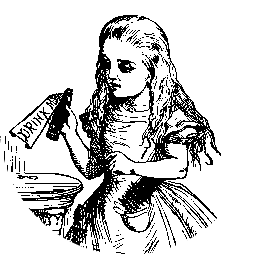
\includegraphics[height=.2\paperheight]{pics/alice}}
\end{frame}

% Diagrams here showing what is going on in the workflow with alice
% and bob labels on the keys.

\begin{frame}
  \minionveryhigh{\color{white}{\color{b-grey}Bob} requests access}
  \bottomhanging{
    \includegraphics<1>[width=\textwidth]{snippets/cyphr-workflow-2}}
  \bottomhanginghigh{
    \includegraphics<2>[width=.85\textwidth]{diagrams/encryption-workflow-2}}
  \bottomright{
\includegraphics[height=.2\paperheight]{pics/bob}}
\end{frame}

\begin{frame}
  \minionveryhigh{{\color{b-purple}Alice} \color{white} authorises {\color{b-grey}Bob}}
  \bottomhanging{
    \includegraphics<1>[width=\textwidth]{snippets/cyphr-workflow-3}}
  \bottomhanginghigh{
    \includegraphics<2>[width=.85\textwidth]{diagrams/encryption-workflow-3}}
  \bottomright{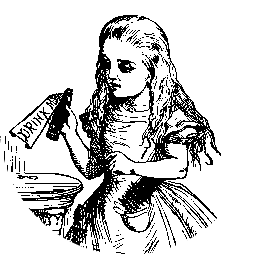
\includegraphics[height=.2\paperheight]{pics/alice}}
\end{frame}

\begin{frame}
  \minionveryhigh{{\color{b-grey}Bob} \color{white} can decrypt {\color{b-pink}data key}}
  \bottomhanginghigh{
    \includegraphics<1>[width=.85\textwidth]{diagrams/encryption-workflow-all}}
  \bottomright{
\includegraphics[height=.2\paperheight]{pics/bob}}
\end{frame}

\begin{frame}
  \minionveryhigh{\color{white}{\color{b-purple}Alice} and
    {\color{b-grey}Bob} \color{white} can decrypt data}
  \begin{tikzpicture}[remember picture, overlay]%
    \node[anchor=north] at
    ($(current page.center) + (0, .24\paperheight)$) {
      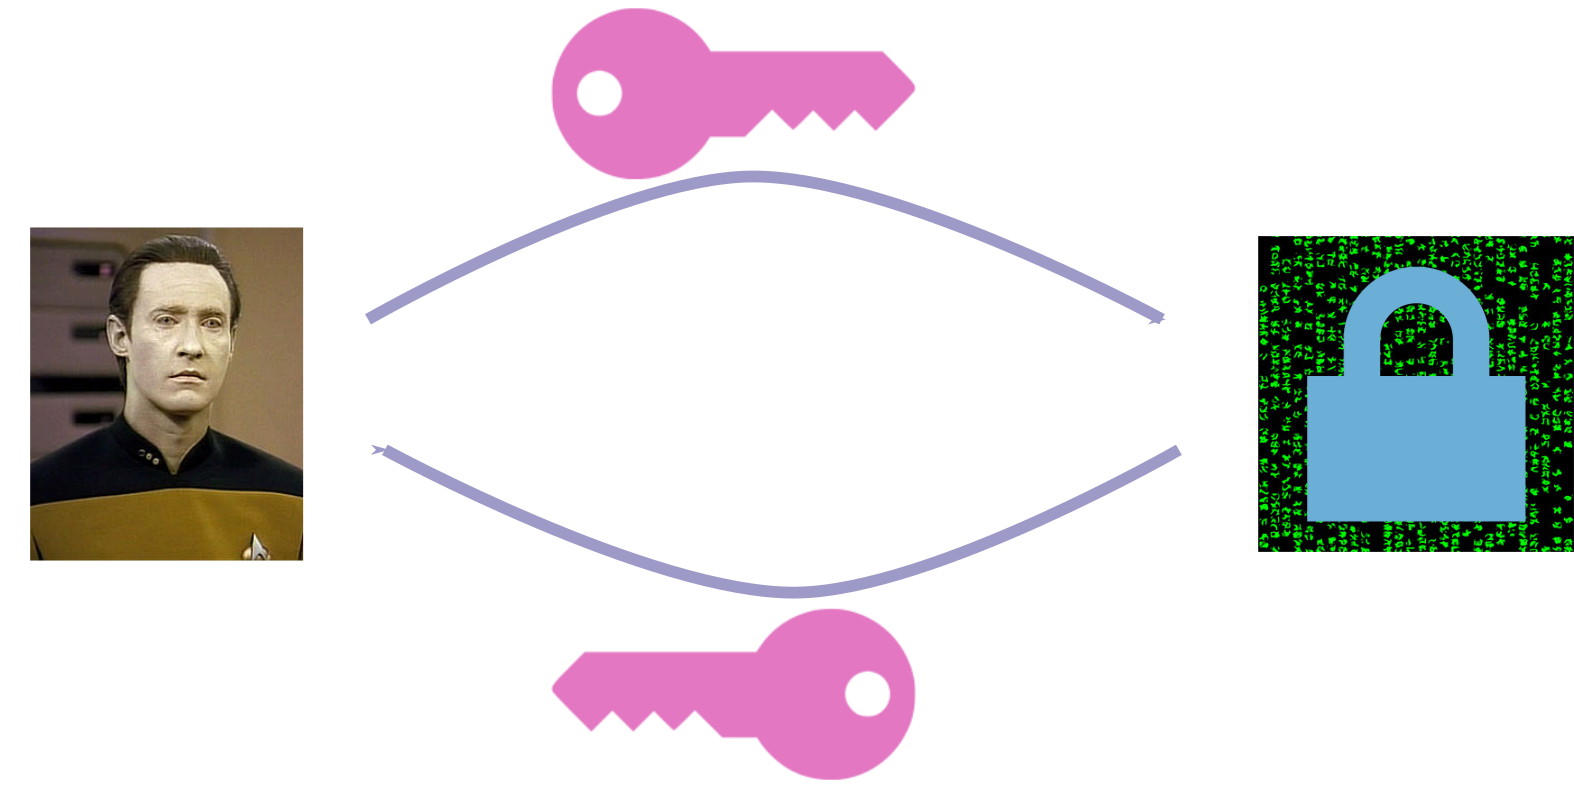
\includegraphics[width=\textwidth]{diagrams/encryption-sym-1}
    };
  \end{tikzpicture}
  \bottomright{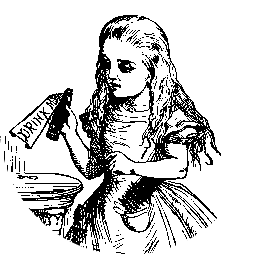
\includegraphics[height=.2\paperheight]{pics/alice}\hspace{.02\paperheight}
\includegraphics[height=.2\paperheight]{pics/bob}}
\end{frame}

\begin{frame}
  \minionhigh{\color{b-pink}How do we\ldots}
  \bottomhanging {
    \begin{minipage}{\textwidth}
      \begin{itemize}
      \item encrypt something?
      \item share keys amongst users?
      \item \ldots so the key is not exposed?
      \item grant access to new people?
      \end{itemize}
    \end{minipage}}
\end{frame}

% Need a summary here still

\begin{frame}
  \hero{\color{b-pink}Danger! Danger!}
  % R is not secure
  % Users are not secure
\end{frame}

\begin{frame}
  \herohigh{\color{b-blue}Summary}
  \bottomhanginglow{
    \begin{minipage}{\textwidth}
      \begin{itemize}
      \item Data distribution \& versioning
      \item Sharing sensitive data
      \end{itemize}
    \end{minipage}}
  \bottomright{
    \begin{minipage}{\textwidth}
      \raggedleft
      \ghrepo{richfitz/datastorr}\\\ghrepo{richfitz/cyphr}
    \end{minipage}
  }
\end{frame}

{
  \setbeamercolor{background canvas}{bg=white}
\begin{frame}
  \inthemiddle{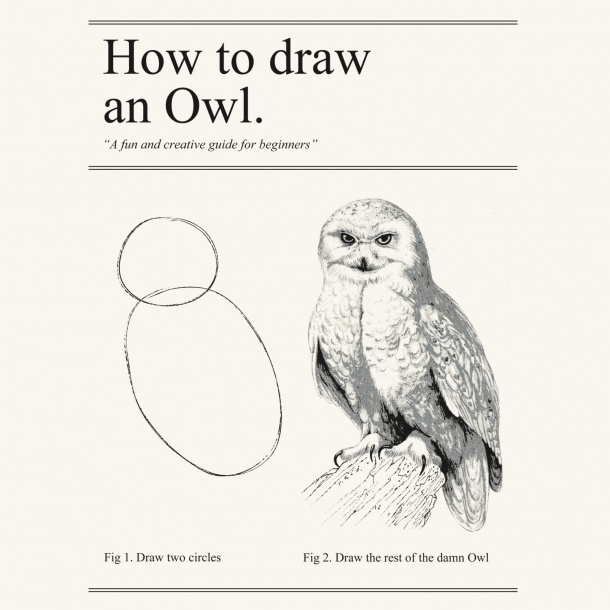
\includegraphics[height=\paperheight]{pics/draw-an-owl}}
\end{frame}
}

\begin{frame}
  \begin{tikzpicture}[remember picture, overlay]%
    \node at
    ($(current page.center) + (0, .15\paperheight)$) {%
      \Huge\it One more thing\ldots
    };
  \end{tikzpicture}
\end{frame}

\begin{frame}
  \begin{tikzpicture}[remember picture, overlay]%
    \node[anchor=west,align=left,font=\Huge\bfseries] (A) at ($(current page.west) + (0.04\paperwidth, .17\paperheight)$) {%
      \color{b-green}Odin
    };
    \node[anchor=north east] at (current page.north east) {%
      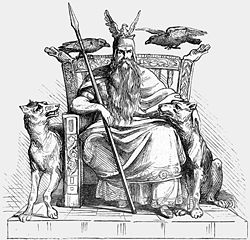
\includegraphics[height=.875\textheight]{pics/odin}
    };
    \node[anchor=south east, align=right,font=\footnotesize] at (current page.south east) {%
      \ghrepo{richfitz/odin}
    };
  \end{tikzpicture}
\end{frame}

\begin{frame}
  \inthemiddle{\includegraphics[height=.8\textheight]{snippets/odin-1}}
  \bottomright{\ghrepo{richfitz/odin}}
\end{frame}

\begin{frame}
  \herohigh{\color{b-blue}Resources}
  \bottomhanginglow {
    \begin{minipage}{\textwidth}
      \tiny
      \begin{itemize}
      \item \ghrepo{richfitz/yvr-2016}
      \item \ghrepo{richfitz/datastorr}
      \item \ghrepo{richfitz/storr}
      \item \ghrepo{richfitz/cyphr}
      \item \ghrepo{traitecoevo/taxonlookup}

      \item \ghrepo{jeroenooms/curl}
      \item \ghrepo{hadley/httr}
      \item \ghrepo{edwindj/daff}
      \item \ghrepo{jeroenooms/openssl}
      \item \ghrepo{jeroenooms/sodium}
      \end{itemize}
    \end{minipage}}
\end{frame}

\end{document}

%%% Local Variables:
%%% mode: latex
%%% TeX-master: t
%%% TeX-engine: xetex
%%% End:
